\documentclass[10pt]{amsart}
\usepackage{geometry}                
\geometry{letterpaper}                  
\usepackage[parfill]{parskip}    
\usepackage{graphicx}
\usepackage{amssymb}
\usepackage{epstopdf}
\usepackage{subfigure}
\DeclareGraphicsRule{.tif}{png}{.png}{`convert #1 `dirname #1`/`basename #1 .tif`.png}
\evensidemargin=0in
\oddsidemargin=0in

\title{ECE 532 Final Project: Voltage Regulator}
\author{John O'Hollaren}

\begin{document}
\maketitle

%%%%%%%%%%%%%%%%%%%%%%%%%%%%%%%%%%%%%%%%%%%%%
\section{Introduction}
In this report I will detail the design of a linear regulator that takes a 5 volt input and outputs 1.5 volts on the output.\\

This report is divided into the following sections:
\begin{enumerate}
\item Design Goals
\item Design Challenges
\item Schematics
\item Simulations
\item Layout
\item Fabrication
\end{enumerate}

\newpage

%%%%%%%%%%%%%%%%%%%%%%%%%%%%%%%%%%%%%%%%%%%%%
\section{Design Goals}

There are several types of linear regulators. Note that drop out depends on a variety of factors, not just the topology (as I show later). My design will use only one power element, and thus falls under the LDO category (even though I am going to optimize it to output 2.5 volts).

\begin{figure}[h]
	\begin{center}
		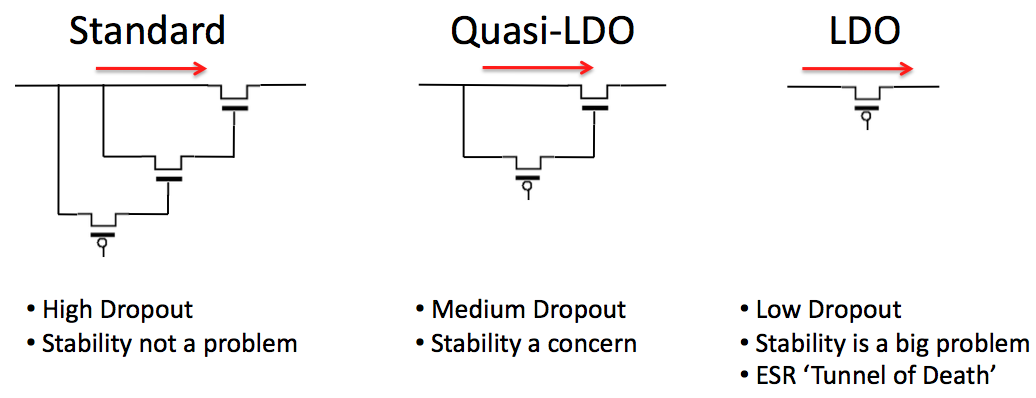
\includegraphics[width=6in]{Media/ldos.png}
	\end{center}
	\caption{Comparison of linear regulator topologies}
	\label{fig:wl}
\end{figure}

I have cut down significantly on the amount of I/O, external power, and references needed from my earlier, more complicated designs. Here is a black box I/O diagram of my final design: 

\begin{figure}[h]
	\begin{center}
		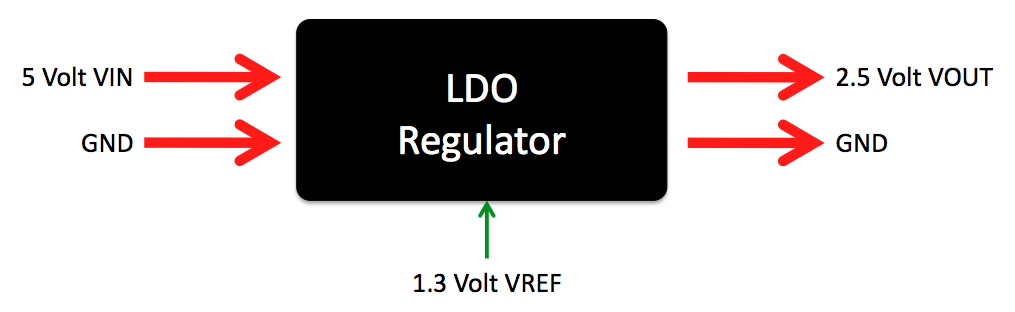
\includegraphics[width=6in]{Media/black.png}
	\end{center}
	\caption{I/O Diagram}
	\label{fig:black}
\end{figure}

Following are the specifications I am designing to. For comparison, I am using the Texas Instruments TLV1171 which is a highly optimized linear regulator that claims 500x lower quiescent power draw over most commercial regulators. Note the TI part outputs 2V, mine will output 2.5 Volts.

\begin{figure}[h]
	\begin{center}
		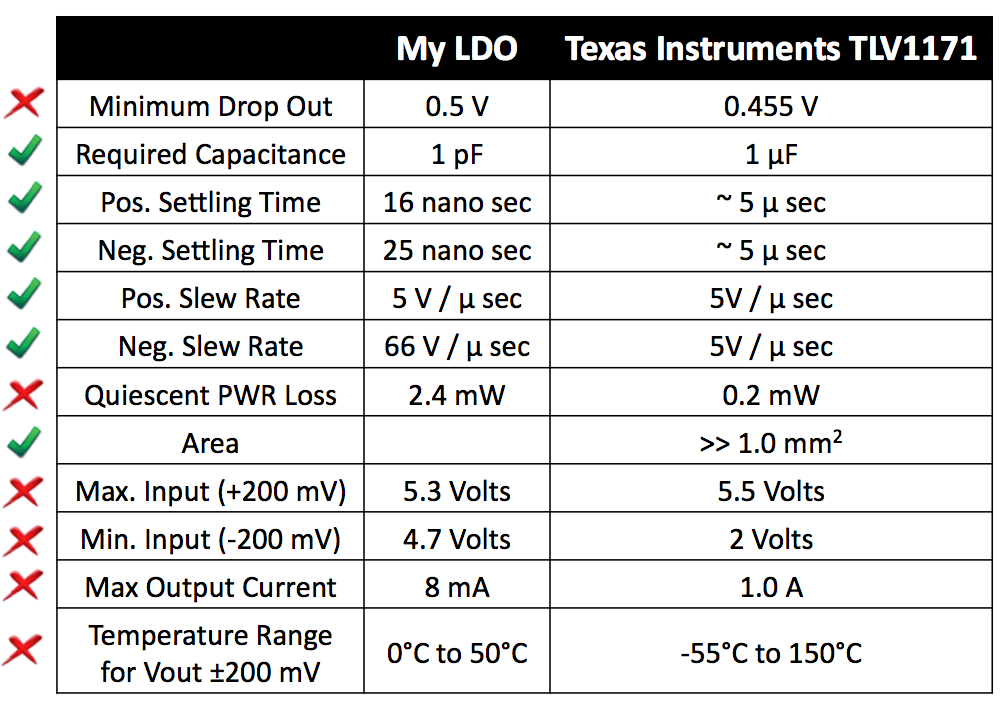
\includegraphics[width=6in]{Media/specs.png}
	\end{center}
	\caption{I/O Diagram. Specs I am able to match or beat are highlighted with green; specs I am not able to match are in red.}
	\label{fig:specs}
\end{figure}

%%%%%%%%%%%%%%%%%%%%%%%%%%%%%%%%%%%%%%%%%%%%%
\section{Design Challenges}

There are a few key challenges I must work around to design this linear regulator. These include a physical limitation with the power MOSFET and process limitations (limited voltage range).

\subsection{Power MOSFET Limitations}

The rule of thumb for analog amplifier design is:
\begin{equation}
\text{Max } I_{DS} = \frac{1 \text{mA}}{ 1 \mu m}
\end{equation}

This suggests that I find the ideal $\frac{W}{L}$ ratio and then scale it up to the current I need. However, there is a problem. As $\frac{W}{L}$, decreases, the $V_{DS}$ of the mosfet becomes a bigger factor. In order to have an efficient regulator, I need a very high $\frac{W}{L}$, which costs a lot of area that I do not have. On the flip side, a larger ratio decreases the size of the controllable linear region, which makes the regulator harder to control.

I want to be able to control my output around 2.5 volts. Therefore, I need to have the linear region be centered around 2.5 volts. Furthermore, I want to be able to push through several mA, so I will choose L = 8u. See the plots to see how I chose my ideal W, which will be 420.

\begin{figure}[h]
	\begin{center}
		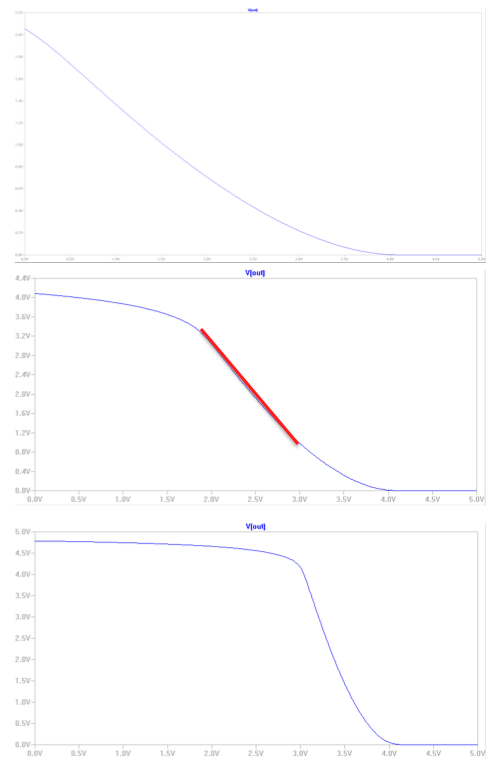
\includegraphics[width=3.6in]{Media/WL.png}
	\end{center}
	\caption{Top: W = 100, Middle: W = 420, Bottom: W = 1000. $V_{DS}$ vs $V_{GS}$ for a single MOSFET using our technology. This is an important graph because $V_{DS}$ determines the output voltage and $V_{GS}$ is what I use to control it. Note the nice linear region around 2.5V for my L = 8u, W = 420u.}
	\label{fig:wl}
\end{figure}

\subsection{Process Limitation: No Negative Voltage}

Use of the negative voltage rail allows a PID controller to be directly implemented in the feedback path. A negative voltage allows me to create an op amp differentiator around a zero point, so that a $V_{out}$ that is too high can directly cause a gate voltage to compensate. My initial design assumed I had access to this negative voltage, so my controller looked like Figure \ref{fig:piedmont}: \\

\begin{figure}[h]
	\begin{center}
		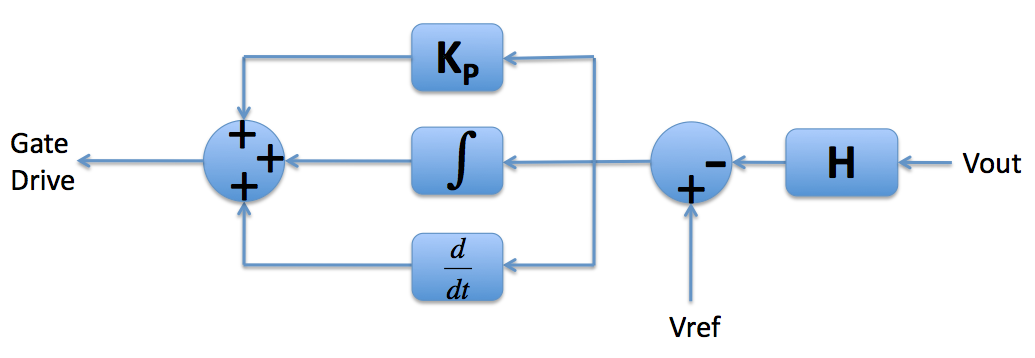
\includegraphics[height=1in]{Media/PID.png}
	\end{center}
	\caption{The initial PID controller I designed.}
	\label{fig:piedmont}
\end{figure}

\begin{figure}[h]
	\begin{center}
		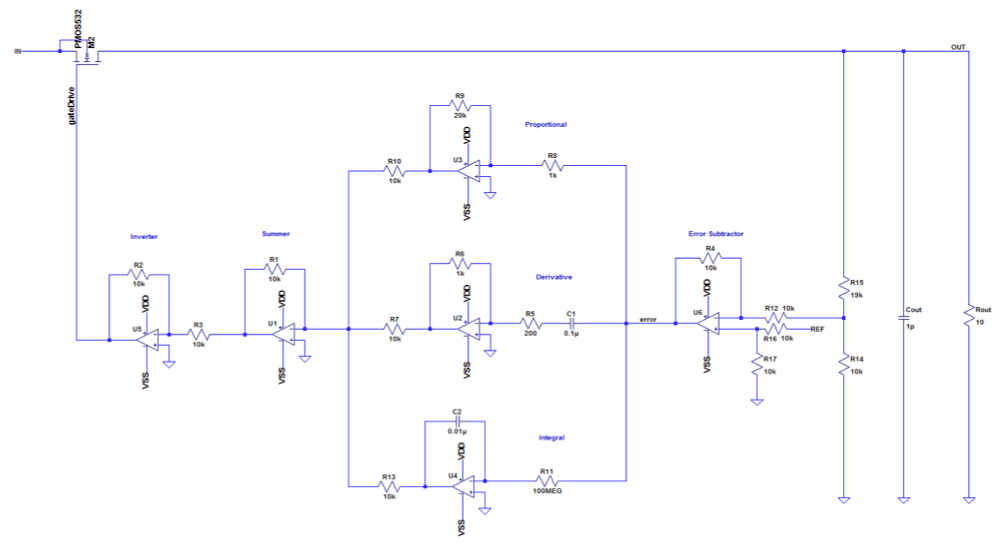
\includegraphics[height=2in]{Media/PID_sc.png}
	\end{center}
	\caption{Using this, I can precisely control the output.}
	\label{fig:pid}
\end{figure}

\begin{figure}[h]
	\begin{center}
		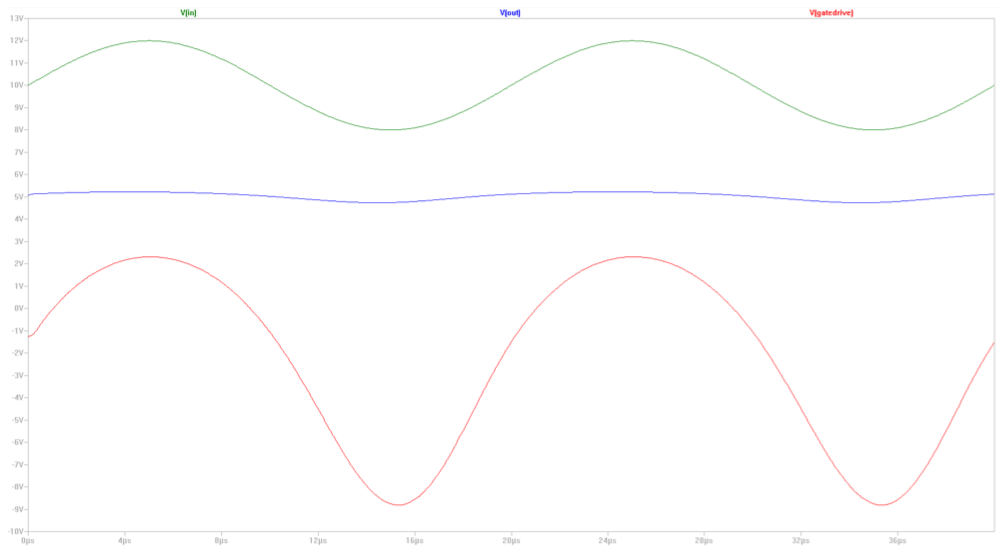
\includegraphics[width=4in]{Media/pidfb.png}
	\end{center}
	\caption{PID controlled output voltage (blue) with a 4V sinusoidal input (green) and the PID controller output (red) to precisely control the blue output and keep it constant.}
	\label{fig:pidfb}
\end{figure}

However, to fabricate my design I will need to have a maximum voltage differential on chip of 5V. Therefore, I do not have access to this negative voltage rail, and I will have to improvise. To solve this I will design a negative feedback proportional-only controller that uses a differential amplifier that does not output a negative voltage. My solution is to output a voltage, 2.5V that can be output without any voltage initialization and also without the gate being needed to be driven negative. The other alternative is a complicated series of circuits and references to step the operating point up, perform the operations, and then step it back down again. Chip manufacturers do this with several hundred transistors, but I will simplify things to complete this project.

\begin{figure}[h]
	\begin{center}
		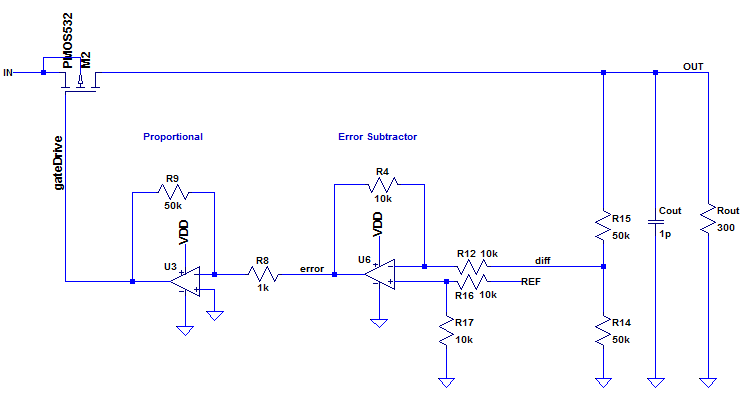
\includegraphics[width=7in]{Media/cleanfinal.png}
	\end{center}
	\caption{A high level view of my final design. Transistor level shown on next page.}
	\label{fig:pidfb}
\end{figure}

\newpage

%%%%%%%%%%%%%%%%%%%%%%%%%%%%%%%%%%%%%%%%%%%%%
\section{Schematics}

Here is the final design:
	\begin{center}
		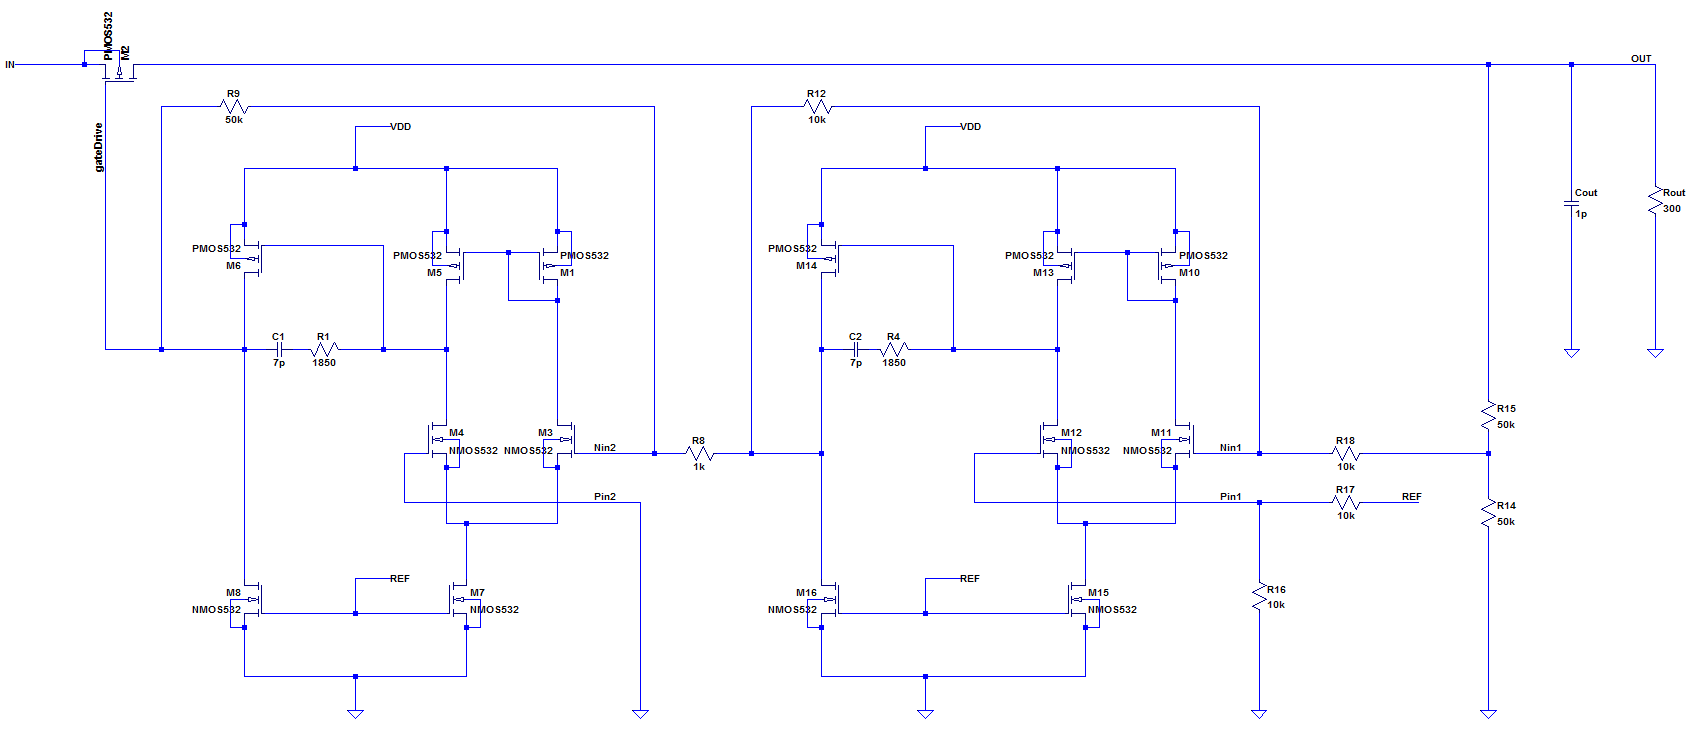
\includegraphics[width=7.0in, angle=90]{Media/design.png}
	\end{center}

\begin{figure}[h]
	\begin{center}
		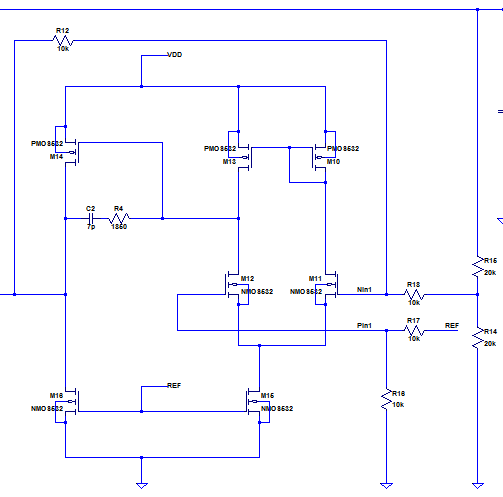
\includegraphics[width=4in]{Media/diff.png}
	\end{center}
	\caption{Close up of error amplifier.}
	\label{fig:pidfb}
\end{figure}

\begin{figure}[h]
	\begin{center}
		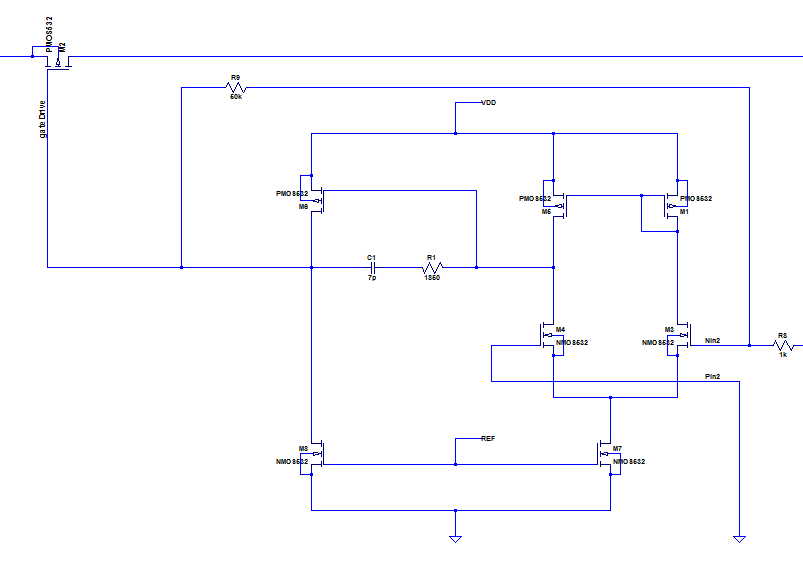
\includegraphics[width=4in]{Media/driver.png}
	\end{center}
	\caption{Close up of inverting amplifier and gate driver.}
	\label{fig:pidfb}
\end{figure}

   .
\newpage

  
%%%%%%%%%%%%%%%%%%%%%%%%%%%%%%%%%%%%%%%%%%%%%
\section{Simulations}

\begin{figure}[h]
	\begin{center}
		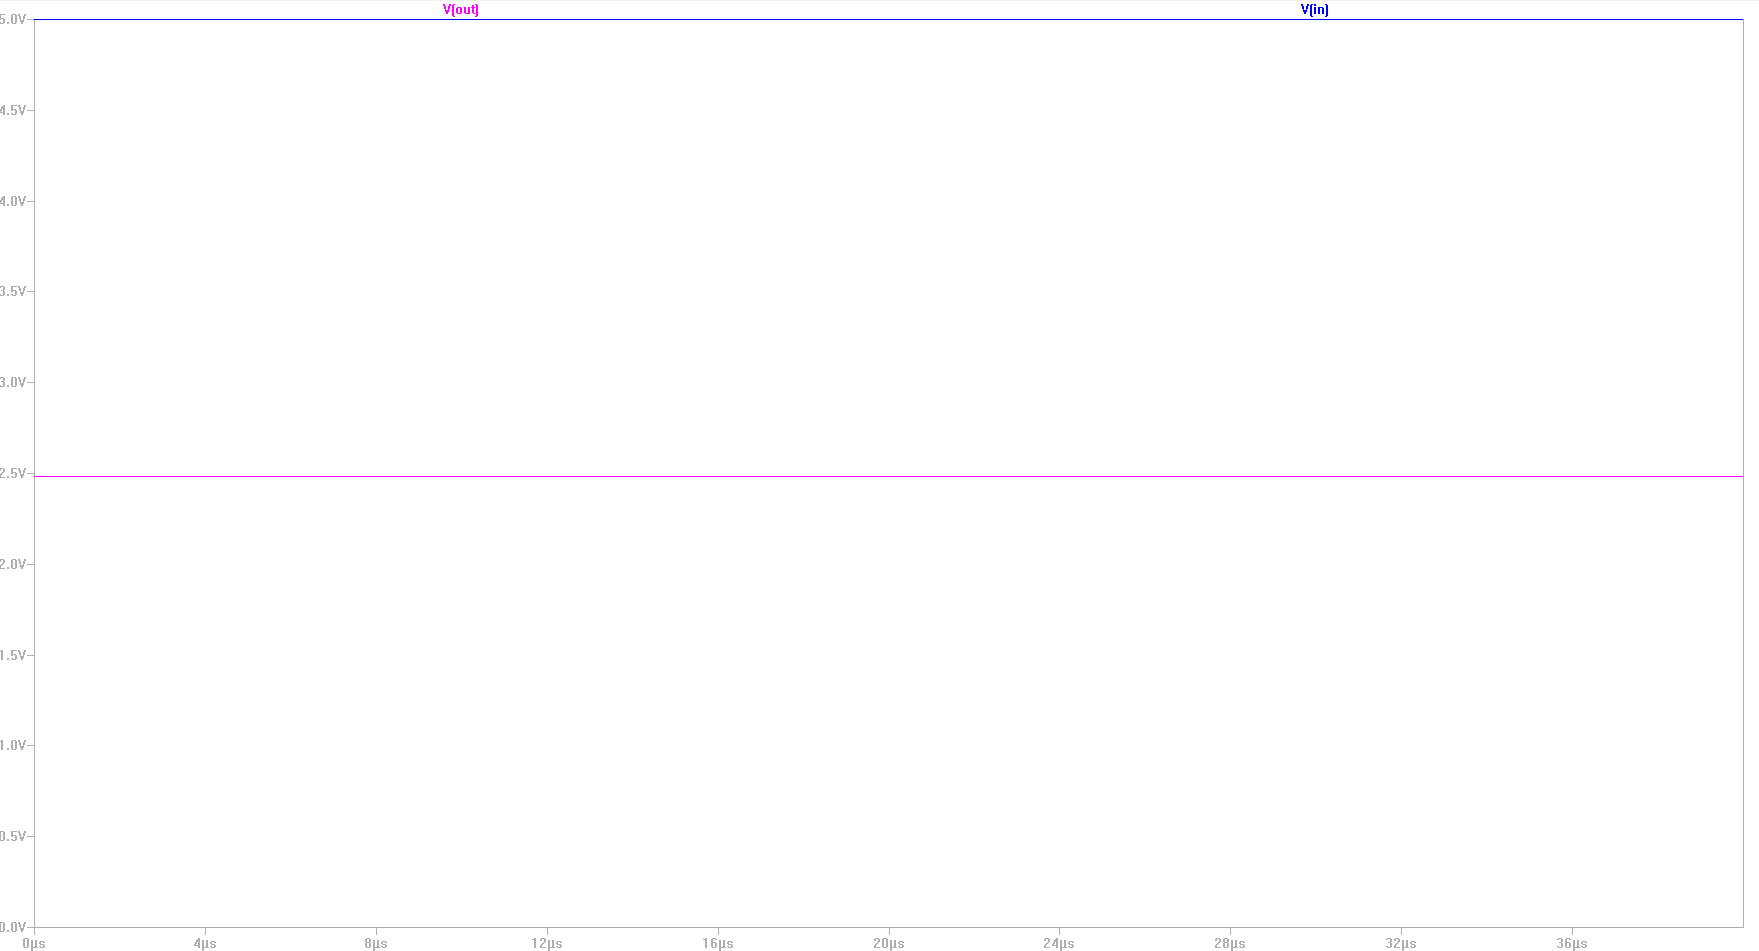
\includegraphics[width=7in]{Media/ss.png}
	\end{center}
	\caption{Steady State Output. $V_{out}$ is 2.5V with the 5V input.}
	\label{fig:pidfb}
\end{figure}

The output is correct to within 0.02 Volts.

\newpage

\begin{figure}[h]
	\begin{center}
		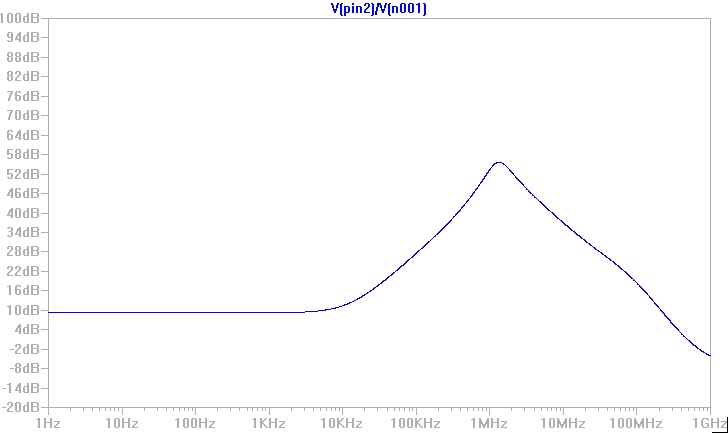
\includegraphics[width=7in]{Media/lg.png}
	\end{center}
	\caption{Loop Gain, $T(s)$.}
	\label{fig:pidfb}
\end{figure}

The loop gain, $T(s)$ is very high, 63 dB. Note in my previous designs the loop gain was about -20 dB. I have greatly improved it here, by over 80 dB. For a negative feedback voltage regulator:\\

Voltage noise on the input is rejected in proportion to $\frac{1}{1 + T(s)} \approx 0$. \\

Voltage disturbances on the load are rejected in proportion to $\frac{1}{1 + T(s)} \approx 0$. \\

The reference voltage is followed in proportion to $\frac{T(s)}{1 + T(s)} \approx 1$. \\

Therefore, since my loop gain, $T(s)$ is very high, voltage and current disturbances should be rejected very well as they are multiplied by 0, and the reference voltage should be followed well as it is multiplied by unity. \\

Note that the above is in the ideal case. I modified my error amplifier to work without a negative rail so I do not actually see nearly the ideal rejection.

\newpage

Output with a sinusoidal input:

\begin{figure}[h]
	\begin{center}
		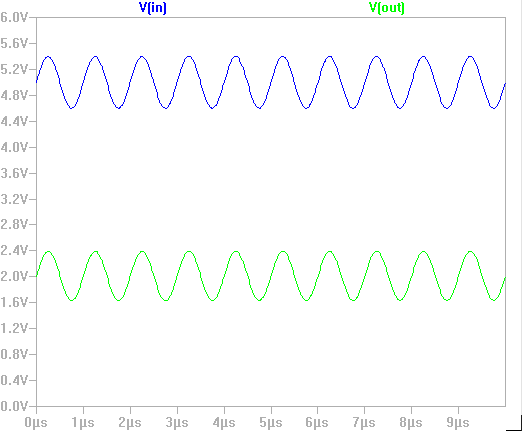
\includegraphics[width=7in]{Media/sin.png}
	\end{center}
	\caption{$V_{out} $ vs $V_{in}$ with a 1V sine wave on the input.}
	\label{fig:pidfb}
\end{figure}

Here is the steady state power loss across the control circuitry:

\begin{figure}[h]
	\begin{center}
		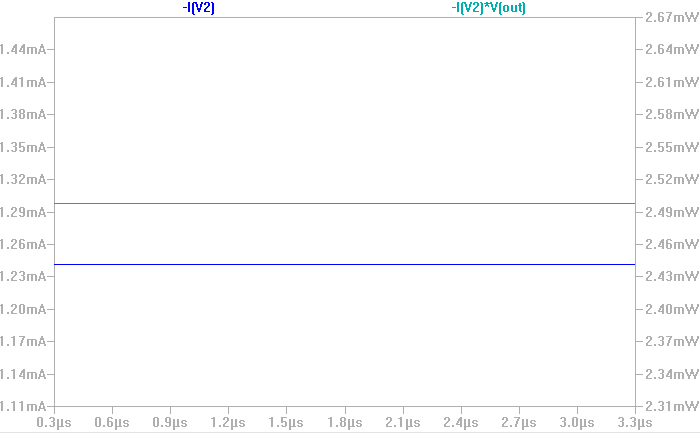
\includegraphics[width=7in]{Media/pwr.png}
	\end{center}
	\caption{Steady state current draw and steady state power loss through control circuitry. The quiescent power loss is 2.4 mW.}
	\label{fig:pidfb}
\end{figure}

\newpage

The positive settling time is 16 nano seconds.

\begin{figure}[h]
	\begin{center}
		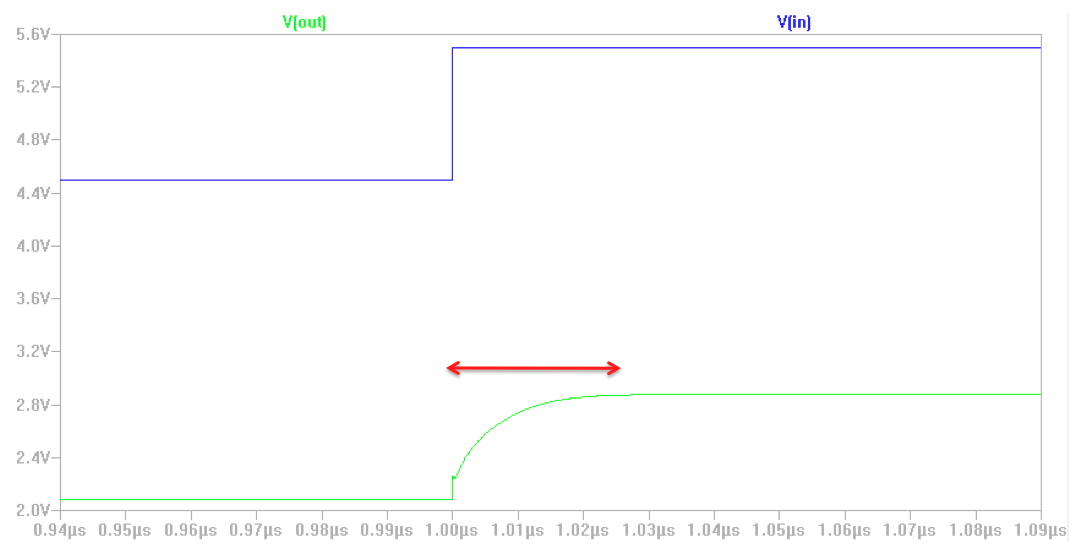
\includegraphics[width=5in]{Media/pos.png}
	\end{center}
	\caption{Positive settling time = 16 ns}
	\label{fig:pos}
\end{figure}

The negative settling time is 25 nano seconds

\begin{figure}[h]
	\begin{center}
		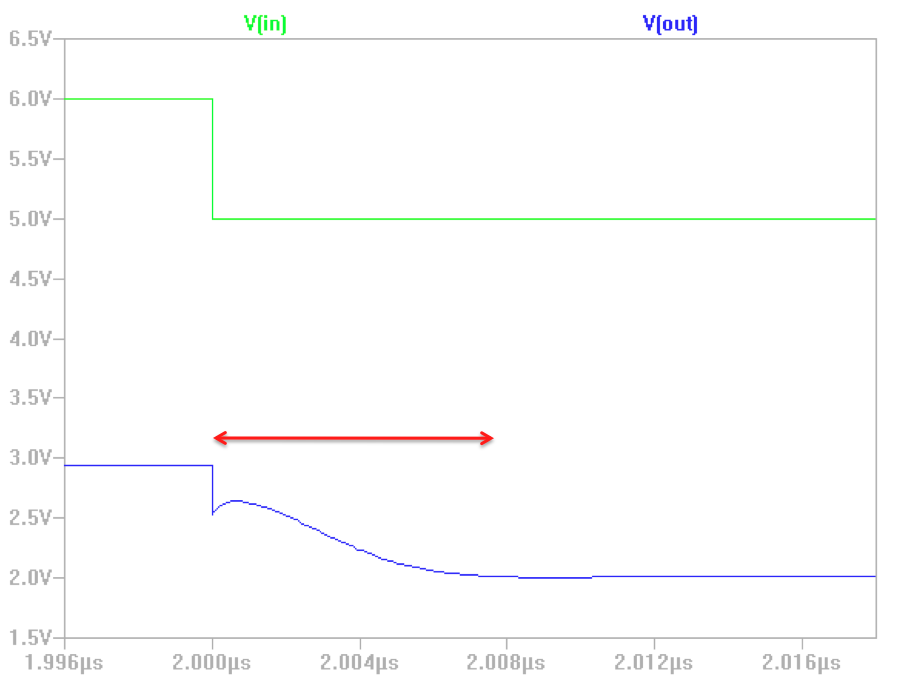
\includegraphics[width=5in]{Media/neg.png}
	\end{center}
	\caption{Negative settling time = 25 ns.}
	\label{fig:neg}
\end{figure}

From the same graphs, I also get the slew rates:

Positive slew rate = \scalebox{1.5}{ $ \frac{5 \text{ Volts}}{\mu \text{ sec}} $ }

Negative slew rate = \scalebox{1.5}{  $\frac{66 \text{ Volts}}{\mu \text{ sec}}$ }

Here is a temperature sweep of my regulator over a 50 degree Celsius range from 25 degrees below ambient to 25 degrees above ambient (0-50). It keeps the output without a 200 mV range of optimal.

\begin{figure}[h]
	\begin{center}
		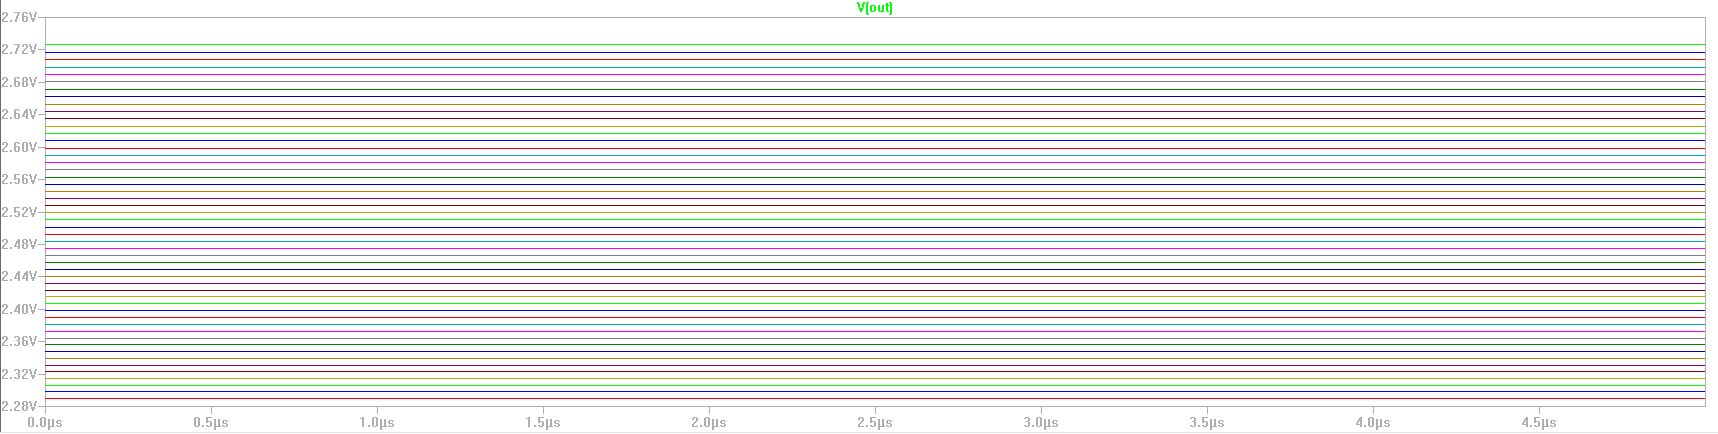
\includegraphics[width=7in]{Media/thermsw.png}
	\end{center}
	\caption{Regulator operation over a range from 0 to 50 degrees Celcius.}
	\label{fig:neg}
\end{figure}

%%%%%%%%%%%%%%%%%%%%%%%%%%%%%%%%%%%%%%%%%%%%%
\section{Layout}

I improved my op amp from homework 4 for this project. Here is my new op amp (the one I used above in simulations) as a schematic and also the layout for it.

\begin{figure}[h]
	\begin{center}
		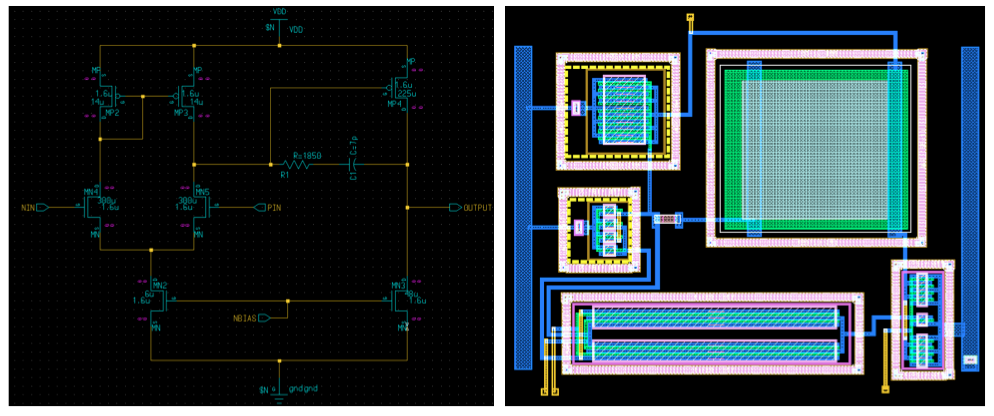
\includegraphics[width=7in]{Media/opamp.png}
	\end{center}
	\caption{My improved op amp.}
	\label{fig:neg}
\end{figure}

\newpage

For the rest of my design, I have several resistors that I need to common centroid. Here is my common centroid scheme:

\begin{figure}[h]
	\begin{center}
		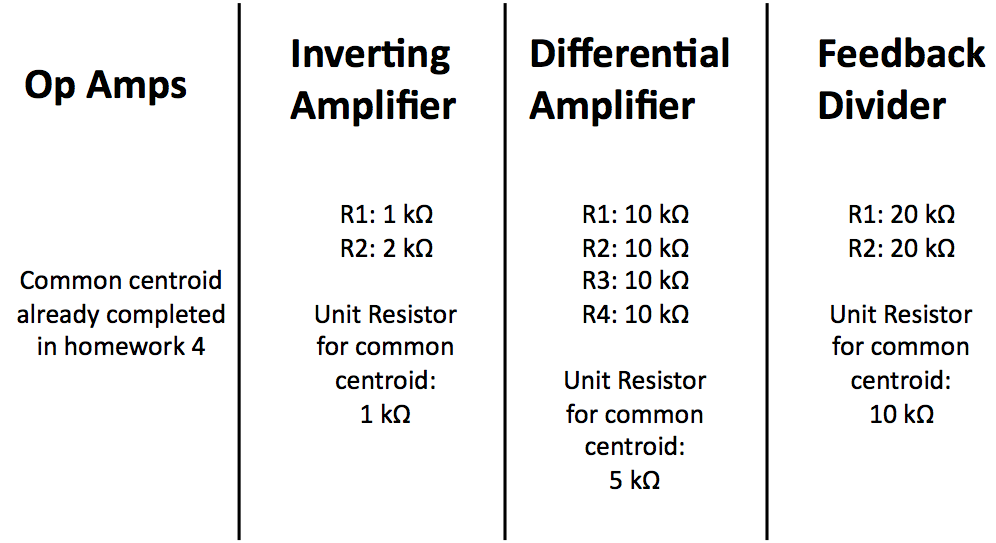
\includegraphics[width=4in]{Media/ccplan.png}
	\end{center}
	\caption{My common centroid scheme.}
	\label{fig:cc}
\end{figure}

%%%%%%%%%%%%%%%%%%%%%%%%%%%%%%%%%%%%%%%%%%%%%
\section{Fabrication}

I am fabricating my project, which is why I have added the extra pads at the top level. I will test the project next semester in the fall when it comes back.

%%%%%%%%%%%%%%%%%%%%%%%%%%%%%%%%%%%%%%%%%%%%%
\section{Conclusion}

I built a full linear regulator in this project. I learned a lot, from how to design a negative feedback controller to the design tradeoffs involved in analog circuits. Almost every decision I made had a pro and a con (such as more current vs more accurate control). The layout showed me how important it is to plan ahead and think of a project modularly.

\end{document}



